\documentclass{article}
\usepackage{graphicx} % Required for inserting images

\documentclass[a4paper, 12pt]{article}%тип документа
\usepackage{xcolor}
%отступы
\usepackage[left=2cm,right=2cm,top=2cm,bottom=3cm,bindingoffset=0cm]{geometry}
\usepackage[pdftex]{lscape}
%Русский язык
\usepackage[T2A]{fontenc} %кодировка
\usepackage[utf8]{inputenc} %кодировка исходного кода
\usepackage[english,russian]{babel} %локализация и переносы
\usepackage{multirow}
%Вставка картинок
\usepackage{wrapfig}
\usepackage{graphicx}
\graphicspath{{Images/}}
\DeclareGraphicsExtensions{.pdf,.png,.jpg}

%Математика
\usepackage{amsmath, amsfonts, amssymb, amsthm, mathtools}

%Заголовокhttps://www.overleaf.com/project/6507f5a4176b25bf05722230

\begin{document}

\begin{titlepage}
	\begin{center}
		{\large МОСКОВСКИЙ ФИЗИКО-ТЕХНИЧЕСКИЙ ИНСТИТУТ (НАЦИОНАЛЬНЫЙ ИССЛЕДОВАТЕЛЬСКИЙ УНИВЕРСИТЕТ)}
	\end{center}
	\begin{center}
		{\large Физтех-школа биологической и медицинской физики}
	\end{center}
	
	
	\vspace{4.5cm}
	{\huge
		\begin{center}
			{\bf Отчёт о выполнении лабораторной работы}\\
			Инфракрасная спектроскопия поглощения. Колебательно-вращательные спектры двухатомных молекул.
		\end{center}
	}
	\vspace{3cm}
	\begin{flushright}
		{\LARGE Авторы:\\ Акимов Максим \\ Кондратюк Наталья \\
			\vspace{0.5cm}
			Б06-206}
	\end{flushright}
	\vspace{3cm}
	\begin{center}
		Долгопрудный 
       \\18 ноября 2024 года
	\end{center}
 
\end{titlepage}

\newpage 
\section{Аннотация}
\paragraph*{Цель работы}: Зарегистрировать и проанализировать ИК-спектры поглощения ряда белков, дерината и соляной кислоты. 
\paragraph*{Задачи}:
\begin{itemize}
    \item Снять спектр поглощения опорного образца (воздуха), спектры поглощения образцов (гемоглобин, альбумин, триптофан, деринат) и скотча.
    \item Снять спектр спектр поглощения HCl, предварительно нагрев до образования паров.
    \item Провести анализ полученных спектров белков.
    \item Сравнить спектр дерината с литературными данными.
    \item Провести анализ вторичной структуры альбумина.
\end{itemize}
\section{Введение}
\subsection{Колебательно-вращательный спектр двухатомной молекулы}\;
\par Зависимость вращательной постоянной от квантового числа v с высокой точностью описывается формулой:
\[B_v = B_e - \alpha_e\left(v+\frac{1}{2}\right),\]
где $\alpha_e$ - константа, которая мала по сравнению с $B_e$, т.к. изменение расстояния между ядрами в результате возбуждения колебательных состояний мало по сравнению с самим межъядерным расстоянием. В итоге колебательная и вращательная энергии молекулы принимают вид:
\[\varepsilon_{j,v} = B_v j(j+1) + w_e \left(v+\frac{1}{2}\right) - w_ex_e\left(v+\frac{1}{2}\right)^2, \text{[cм}^{-1}\text{]} \]
\par Правила отбора для комбинированных переходов практически те же, что и для колебательных и вращательных переходов в отдельности:
\[\Delta v = \pm1,\pm2,\pm3,...;  \Delta j = \pm1.\]

\begin{wrapfigure}{r}{0.25\textwidth}
    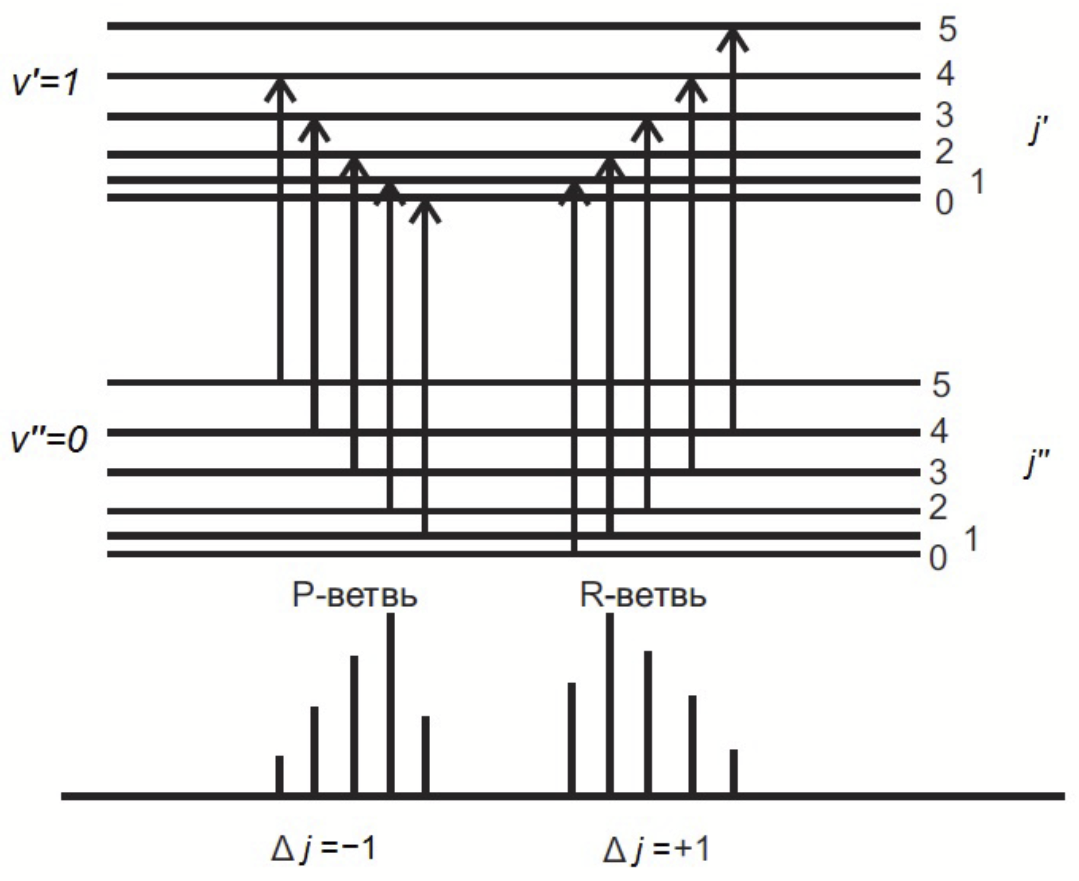
\includegraphics[width=\linewidth]{теория.png}
    \caption{P- и R-ветви колебательно-вращательного спектра двухатомной молекулы}
    \label{колебательные уровни двухатомной молекулы}
\end{wrapfigure}
\par Излучательные переходы с $\Delta j = 0$ практически не имеют места для двухатомных молекул, т.е. колебательный переход всегда сопровождается вращательным.
\par Колебательно-вращательные полосы (рис. \ref{колебательные уровни двухатомной молекулы}) состоят из R-ветви - совокупности линий, для которых выполняется условия $\Delta j = \text{+1}$ и из P-ветви, где $\Delta j = \text{-1}$. Между сериями P и R-ветвей находится так называемый нулевой промежуток (начало полосы) $\nu_0$. Он соответствует чисто колебательному переходу $j^{''} = 0 -> j^{'} = 0$, который для большинства двухатомных молекул запрещен правилами отбора. Поэтому отсчет P-линий начинается с $j = j^{''} = 1$. Ветвь R всегда расположена со стороны больших частот от $\nu_0$, а первая наблюдаемя линия соответсвует $j = 0$.
\newpage

\subsection{Интенсивности линий в спектре}\;
\par Для равновесных условий заселенность энергетических уровней
определяется распределением Больцмана:
\[n_i = n_0 \frac{g_i}{g_0} \exp{\left(-\frac{\Delta E_i}{kT}\right)},\]
$n_i, n_0$ - число молекул в i-m и нулевом энергетическом состояниях, $\Delta E_i$ - разница энергий между этими состояниями, $g_i, g_0$ - статистические веса состояний, k - постоянная Больцамана, T - температура.
\par Статистический вес вращательного состояния равен $g = 2j+1$, а распределение по вращательным состояниям имеет вид:
\[n_j = n_0(2j+1)\exp{\left(-\frac{\Delta E_i}{kT}\right)}\]
Таким образом, рост интенсивности спектральных линий при малых j связан с линейным ростом степени вырождения вращательных уровней, а спад определяется экспоненциально низкой заселенностью высоких энергетических уровней.

\subsection{FTIR-спектроскопия}\;
\begin{figure}[h!]
    \centering
    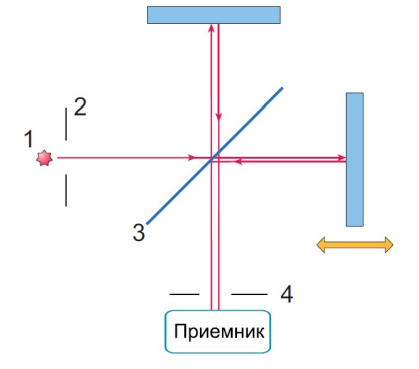
\includegraphics[width=0.5\linewidth]{scheme.png}
    \caption{Принципиальная схема прибора на основе интерферометра Майкельсона.}
    \label{прицип установки}
\end{figure}
\par В основе установки интерферометр (здесь - Майкельсона). При монохроматическом освещении входного отверстия интерферометра и при равномерном перемещении подвижного зеркала со скоростью v, приемником излучения, расположенным за выходной диафрагмой интерферометра, будет регистрироваться переменных сигнал Ф(х), соответсвующий прохождению через выходную диафрагму интерферометра максимумов и минимумов интреференционной картины:
\[\text{Ф}(x) \sim B\cos^2{(\pi \nu x)} = \frac{B}{2}(1+\cos{(2\pi \nu x)})\]
\par Здесь B - яркость светового потока на входе в интерферометр, х - разность хода, равная удвоенной величине перемещения зеркала и линейно зависящая от времени (при равномерной скорости движения зеркала), $\nu$ - частота излучения в $\text{см}^{-1}$. Тогда переменная составляющая зарегистрированный сигнал равна:
\[\text{Ф}(x) = \text{Ф}_0 \cos{(2\pi \nu x)} = \text{Ф}_0\cos{(2\pi ft)},\]
где $f = v\nu = \frac{v}{\lambda}$ - частота модуляции. Таким образом, при монохроматическом освещении входной щели интерферометра приемник излучения регистрирует синусоидальный сигнал.\par
Если входное отверстие интерферометра освещено излучением с непрерывным спектром, занимающим область частот от $\nu_1$ до $\nu_2$, то сигнал, регистрируемый приемником, имеет вид:
\[\text{Ф}(x) \sim \int_{\nu_1}^{\nu_2} B_{\nu}(\nu)\cos{(2\pi \nu x)d\nu},\]
где $B_{\nu}(\nu)$ - спектральная яркость. Данное выражение является фурье-преобразованием функции $B_{\nu}(\nu)$. Спектральная яркость излучения восстанавливается с помощью обратного преобразования Фурье зарегистрированного сигнала:
\[B_{\nu}(\nu) = \int_{-\infty}^{+\infty} \text{Ф}(x) \text{D}(x)\cos{(2\pi \nu x)} dx\]
\section{Экспериментальная установка}\;
\begin{figure} [h!]
    \centering
    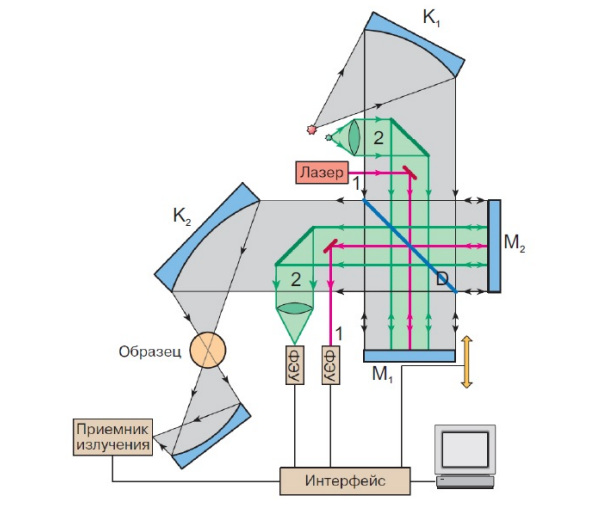
\includegraphics[width=0.5\linewidth]{прибор.png}
    \caption{Схема устройства фурье-спектрометра}
    \label{экспериментальная установка}
\end{figure}
\par Типичная оптическая схема Фурье-спектрометра использует интерферометр Майкельсона. Прошедший через входную диафрагму свет падает на коллиматорное зеракло $K_1$ и параллельным пучком направляется на светоделитель $D$.
Светоделитель обычно представляет собой прозрачную плоскопараллельную пластину с покрытием. Идеальный светоделитель должен отражать и пропускать ровно по $50\%$ света и не иметь поглощения во всей спектральной области
работы прибора. После светоделителя прошедший и отражённый пучки попадают на отражающие зеркала $M_1$ и $M_2$. Выходящее из интерферометра излучение фокусируется зеркальным
объективом $K_2$ в месте, куда помещается образец. После этого свет фокусируется на приёмнике излучения.
\par
Важным элементом оптической схемы является система измерения разности хода между
зеркалами интерферометра. Для этой цели в него вводится излучение одномодового лазера
(обычно это лазер He-Ne). После прохождения через интерферометр монохроматический пучок генерирует при движении зеркала синусоидальный сигнал на специальном приёмнике.
\section{Результаты и обсуждение}
\subsection{Спектр скотча}\;
\par Согласно методическому пособию были подготовлены порошки белков и жидкие образцы. Все измерения необходимо было регистрировать на скотче, плотно засыпав клейкую часть веществом - даже в таком случае на спектре есть возможность снять спектр скотча. Для исключения лишних пиков проведём регистрацию спектра скотча (рис. \ref{скотч}).
\begin{figure}[h!]
\centering
    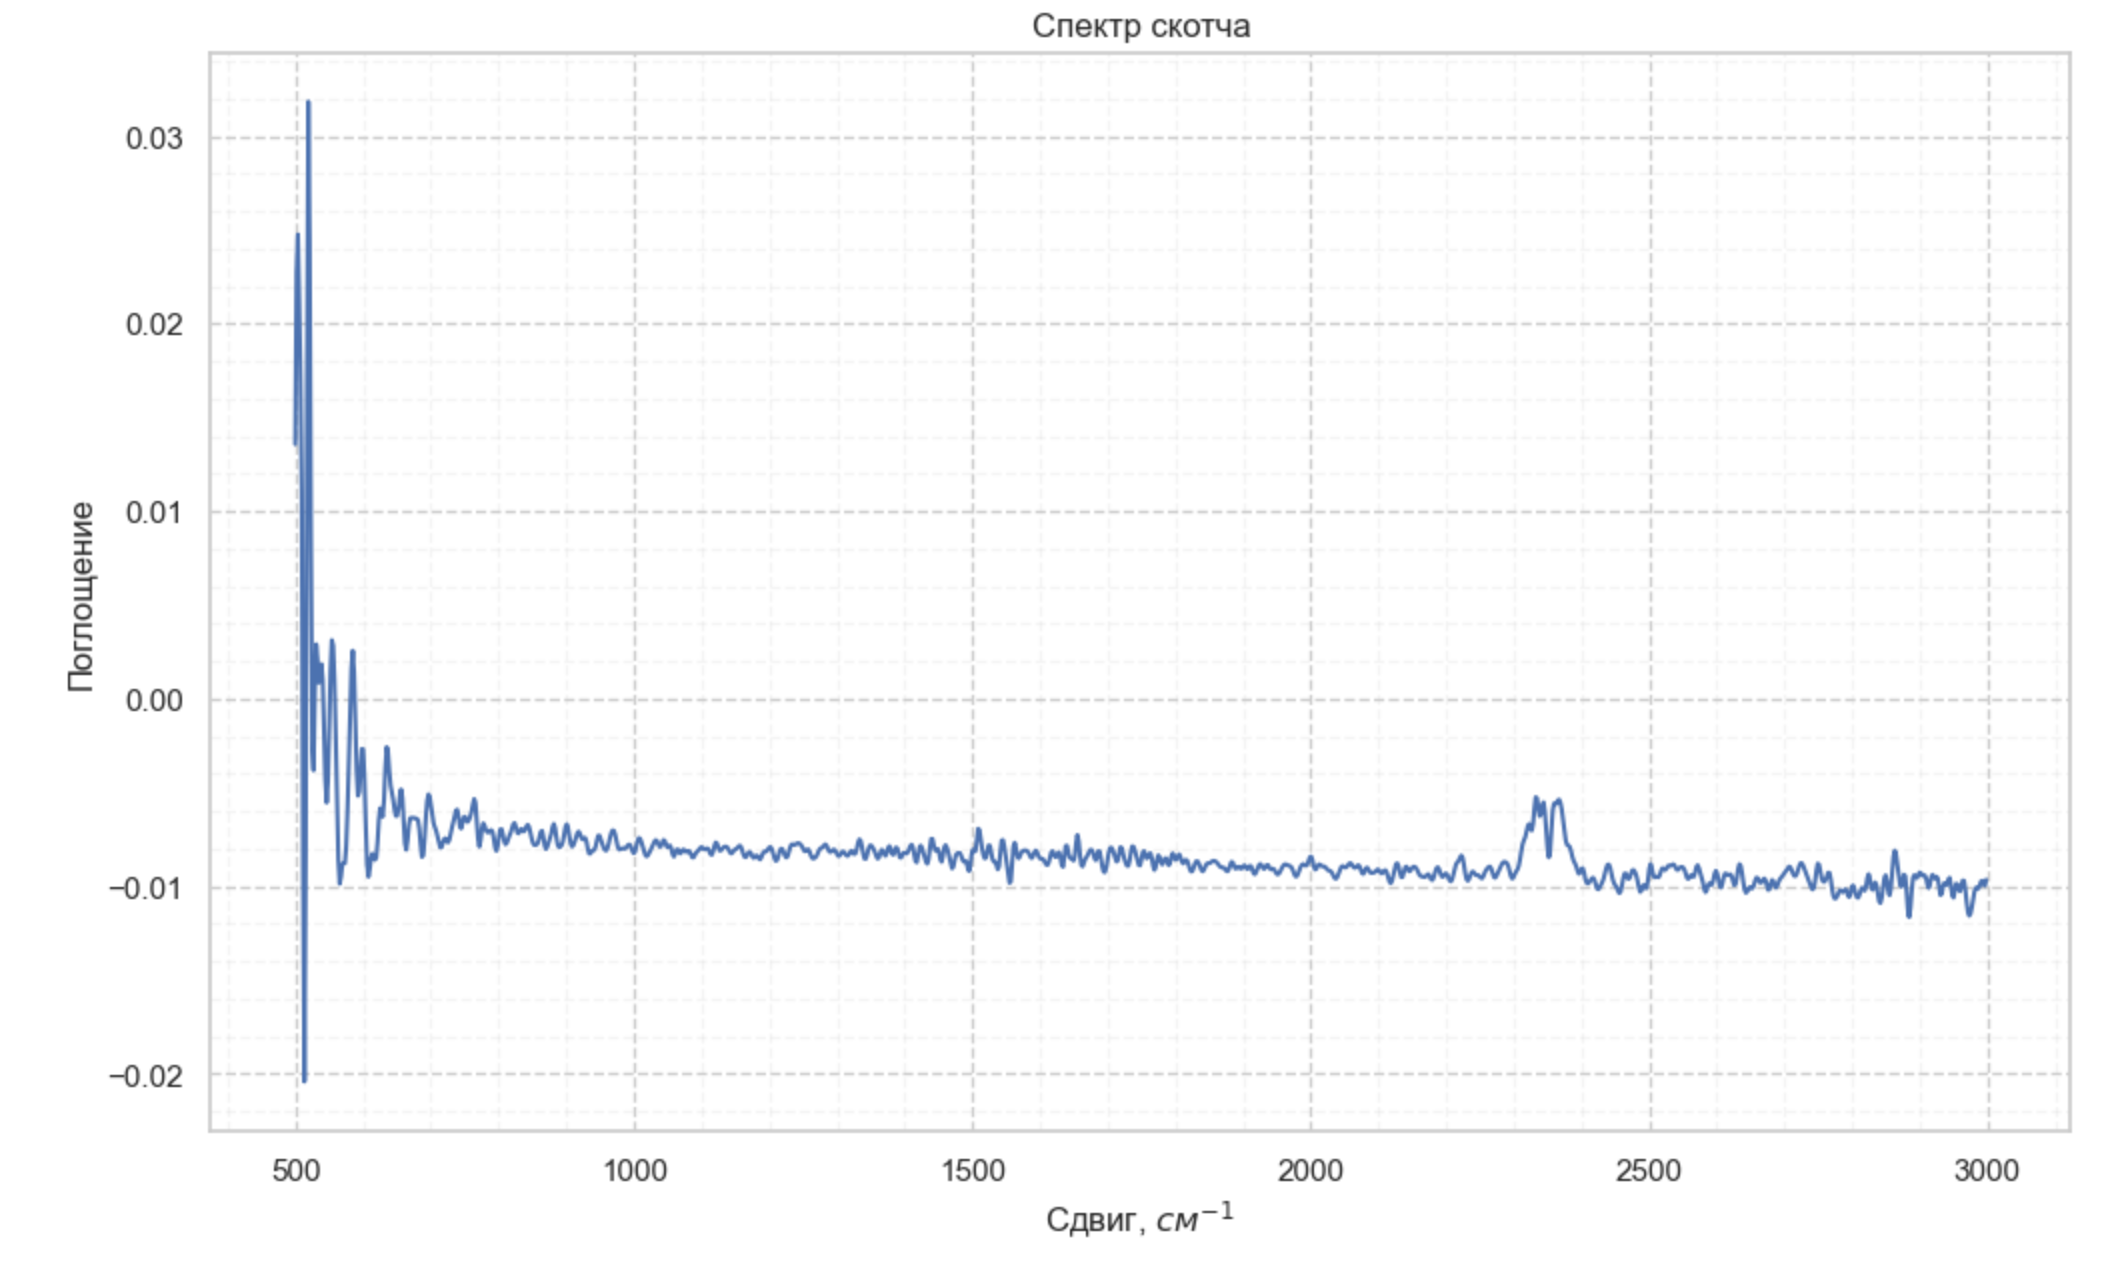
\includegraphics[width=0.8\linewidth]{Images/скотч.png}
    \caption{Спектр поглощения скотча}
    \label{скотч}
\end{figure}
\par Здесь мы столкнулись с проблемой регистрации спектров на данной установке - отсутствие явных чётких пиков поглощения для образцов на скотче и самого скотча. Дальнейшие измерения проводились с порошком, плотно насыпанным в лунку детектора. Также, не удалось установить пик поглощения скотча для нормировки следующих спектров.
\subsection{Анализ FTIR спектров белков}\;
\par В работе было проведено снятие спектров следующих порошков: альбумина, гемоглобина и триптофана.

Для начала проанализируем полученные спектры, сравнив основные пики, называемые Амидами с литературными данными.

\textbf{БСА}

Снятый спектр и его усечённый вариант представлены на Рис. \ref{БСА} и Рис. \ref{БСА усечённое}, соответственно. 

\begin{figure}[h!] 
        \centering
        \minipage{0.5\textwidth}
        \centering
            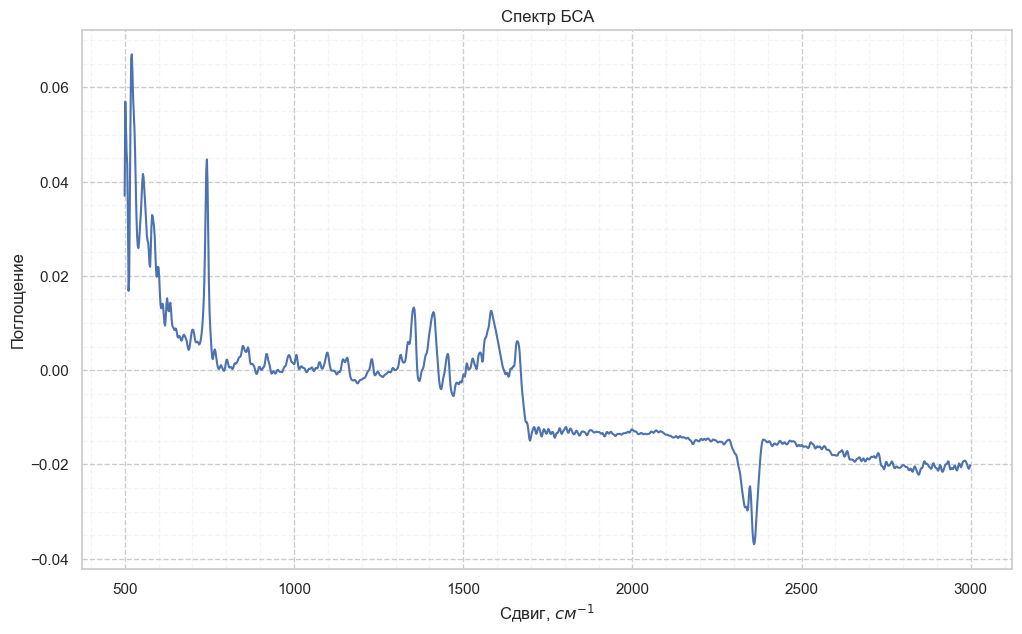
\includegraphics[width=0.9\linewidth]{Images/БСА.png}
                 \caption{Спектр поглощения БСА (порошок)}
                 \label{БСА}
        \endminipage\hfill
        \minipage{0.5\textwidth}
        \centering
             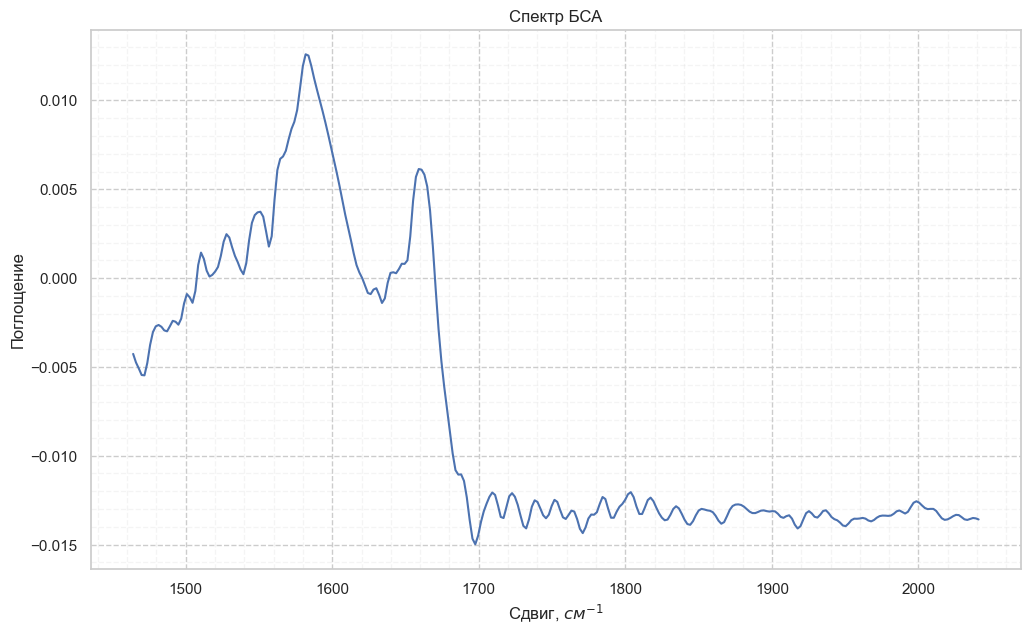
\includegraphics[width=0.9\linewidth]{Images/БСА усечённое.png}
                 \caption{Усечённый вариант спектра с интересующими пиками}
                 \label{БСА усечённое}
        \endminipage
\end{figure}

Сравним полученные данные пиков с теоретическими (взятых из [1]). Соберём все численные значения в Таблице \ref{БСА_табл}:

\begin{table}[h!]
\centering
\caption{Сравнение теоретических и экспериментальных пиков БСА.}
\begin{tabular}{|l|l|l|}
\hline
 & Теоретический диапазон & Экспериментальное значение \\ \hline
Пик Амид I, см$^{-1}$ & 1600 - 1690 & 1659,05 \\ \hline
Пик Амид II, см$^{-1}$& 1480 - 1575 & 1581,88 \\ \hline
\end{tabular}
\label{БСА_табл}
\end{table}

\textbf{Гемоглобин}

Повторим те же самые эксперименты с гемоглобином на Рис. \ref{Гемоглобин} и Рис. \ref{Гемоглобин усечённое}. 

\begin{figure}[h!] 
        \centering
        \minipage{0.5\textwidth}
        \centering
            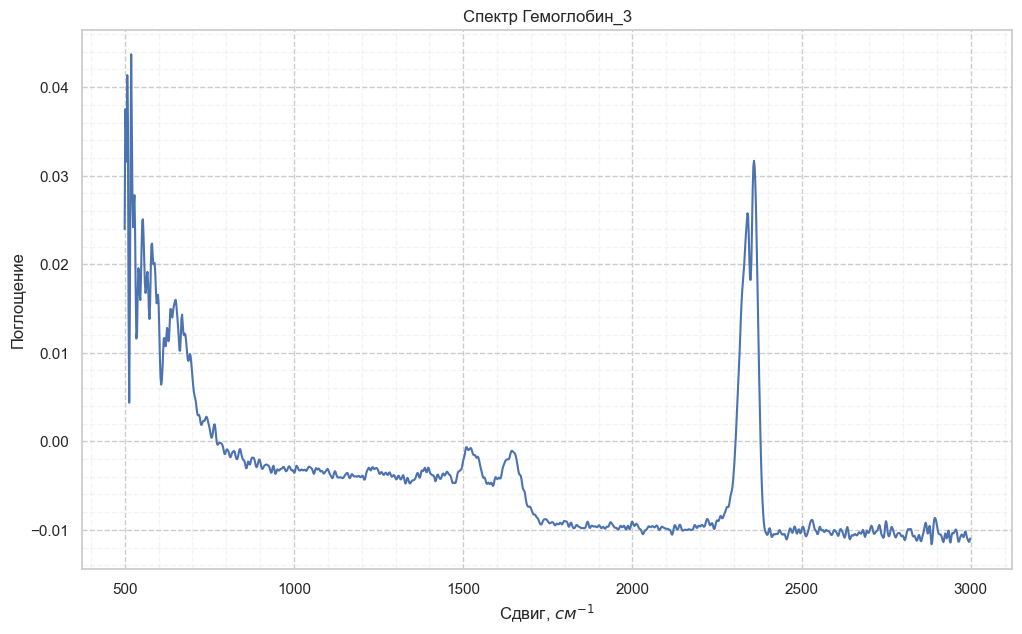
\includegraphics[width=0.9\linewidth]{Images/Гемоглобин.png}
                 \caption{Спектр поглощения БСА (порошок)}
                 \label{Гемоглобин}
        \endminipage\hfill
        \minipage{0.5\textwidth}
        \centering
             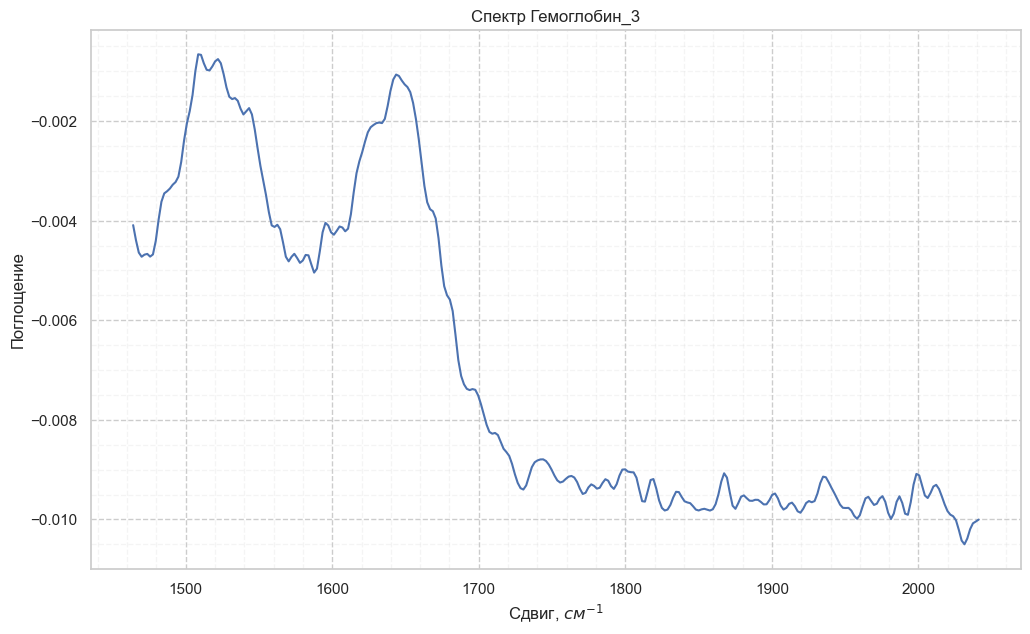
\includegraphics[width=0.9\linewidth]{Images/Гемоглобин усечённое.png}
                 \caption{Усечённый вариант спектра с интересующими пиками}
                 \label{Гемоглобин усечённое}
        \endminipage
\end{figure}

Сравним полученные данные пиков с теоретическими (взятых из [1]) в Таблице \ref{Гемоглобин_табл}:

\begin{table}[h!]
\centering
\caption{Сравнение теоретических и экспериментальных пиков БСА.}
\begin{tabular}{|l|l|l|}
\hline
 & Теоретический диапазон & Экспериментальное значение \\ \hline
Пик Амид I, см$^{-1}$ & 1600 - 1690 & 1643,61 \\ \hline
Пик Амид II, см$^{-1}$& 1480 - 1575 & 1508,57 \\ \hline
\end{tabular}
\label{Гемоглобин_табл}
\end{table}

\textbf{Триптофан}

И ещё раз проведём те же самые эксперименты с триптофаном на Рис. \ref{Триптофан} и Рис. \ref{Триптофан усечённое}. 

\begin{figure}[h!] 
        \centering
        \minipage{0.5\textwidth}
        \centering
            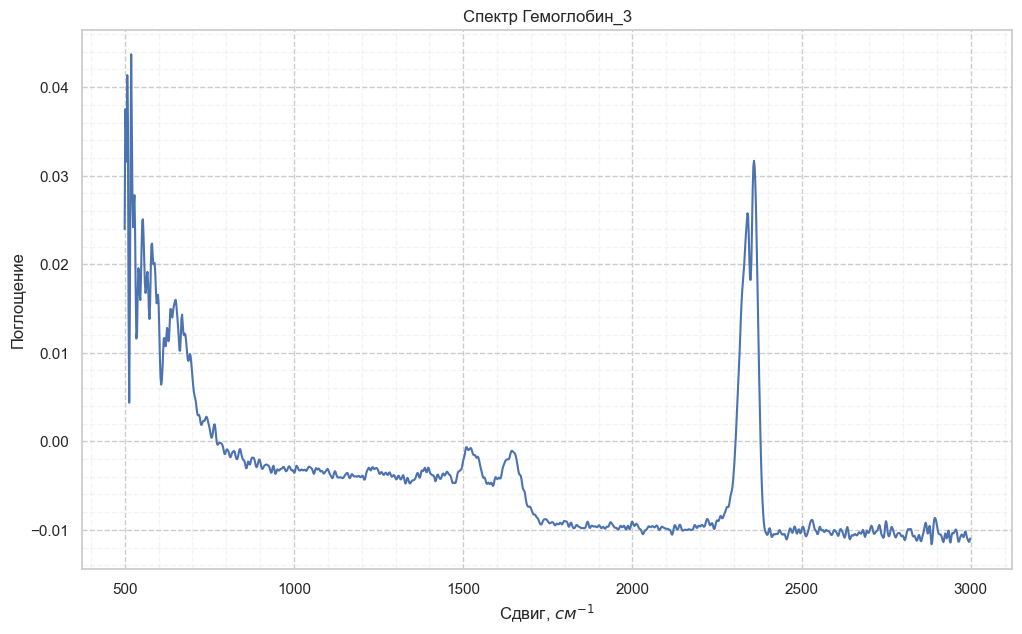
\includegraphics[width=0.9\linewidth]{Images/Гемоглобин.png}
                 \caption{Спектр поглощения триптофана (порошок)}
                 \label{Триптофан}
        \endminipage\hfill
        \minipage{0.5\textwidth}
        \centering
             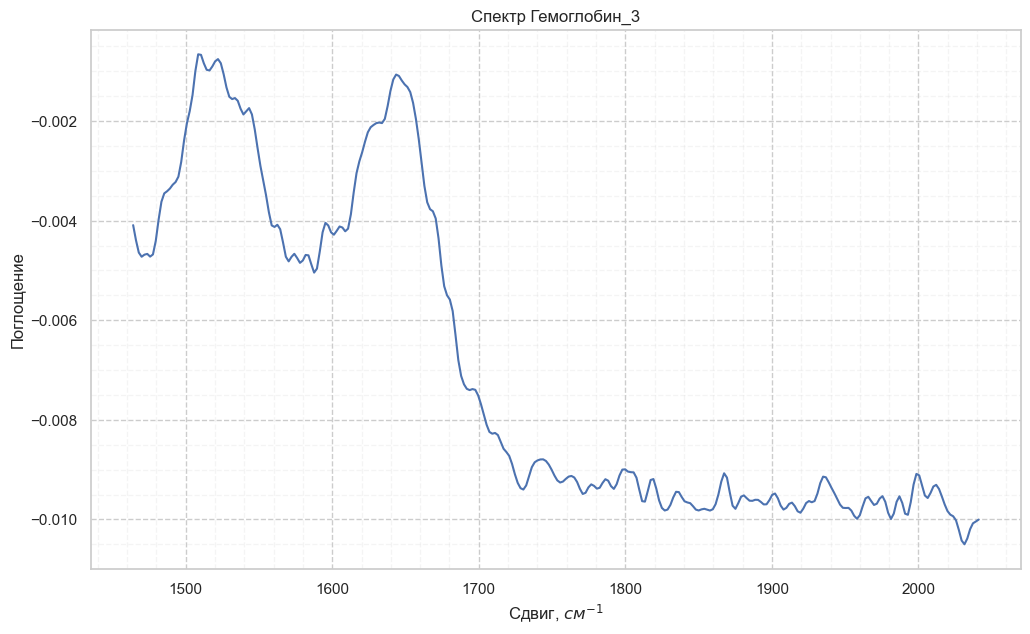
\includegraphics[width=0.9\linewidth]{Images/Гемоглобин усечённое.png}
                 \caption{Усечённый вариант спектра с интересующими пиками}
                 \label{Триптофан усечённое}
        \endminipage
\end{figure}

Сравним полученные данные пиков с теоретическими (взятых из [1]) в Таблице \ref{Триптофан_табл}:

\begin{table}[h!]
\centering
\caption{Сравнение теоретических и экспериментальных пиков триптофана.}
\begin{tabular}{|l|l|l|}
\hline
 & Теоретический диапазон & Экспериментальное значение \\ \hline
Пик Амид I, см$^{-1}$ & 1600 - 1690 & 1662,9 \\ \hline
Пик Амид II, см$^{-1}$& 1480 - 1575 & 1581,88 \\ \hline
\end{tabular}
\label{Триптофан_табл}
\end{table}

\textbf{БСА и гемоглобин}
Теперь будем проводить сравнительные анализы спектров. Начнём со спектров БСА и Гемоглобина. 

\begin{figure}[h!]
\centering
    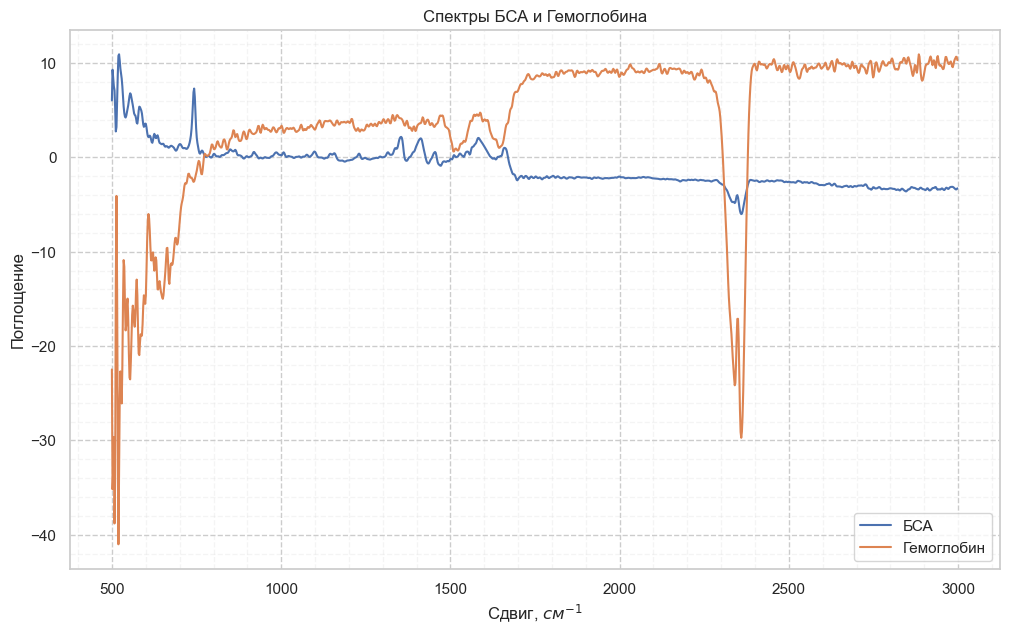
\includegraphics[width=0.8\linewidth]{Images/БСА+Гем.png}
    \caption{Спектры БСА и гемоглобина}
    \label{БСА и Гем}
\end{figure}

На Рис. \ref{БСА и Гем} можно отметить, что в малочастотной области можно наблюдать пики, соответствующие так называемым "отпечаткам пальцев", которые у каждой молекулы свои. В области Амид 1 и Амид 2 можно так же отметить сдвиг пиков БСА вправо, относительно гемоглобина.


\textbf{БСА и триптофан}
Сравним теперь спектры БСА и триптофана (Рис. \ref{БСА и Триптофан}).

\begin{figure}[h!]
\centering
    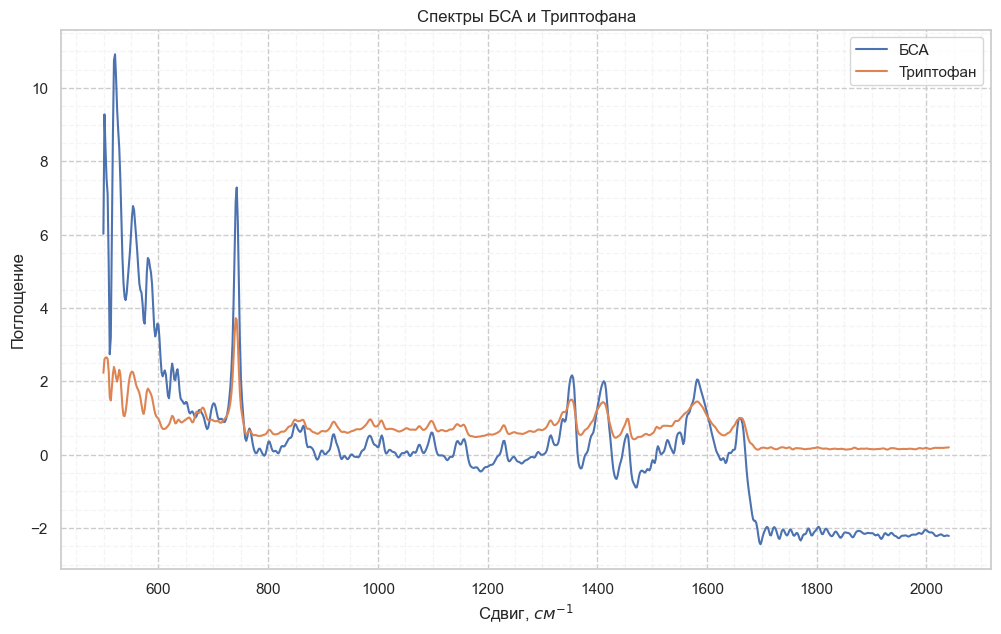
\includegraphics[width=0.8\linewidth]{Images/Триптофан и БСА.png}
    \caption{Спектры БСА и триптофана}
    \label{БСА и Триптофан}
\end{figure}

Можно заметить, что спектры очень похожи и отличаются лишь интенсивностью. И триптофан, и БСА абсолютно совпадают по пику Амида 2: 1581,88 см$^{-1}$. Пики Амида 1 также находятся крайне близко: 1662,9 см$^{-1}$ и 1659,05 см$^{-1}$. Таким образом, можно с уверенностью говорить, что БСА определённо содержит триптофан.  

\textbf{Гемоглобин и триптофан}

\begin{figure}[h!]
\centering
    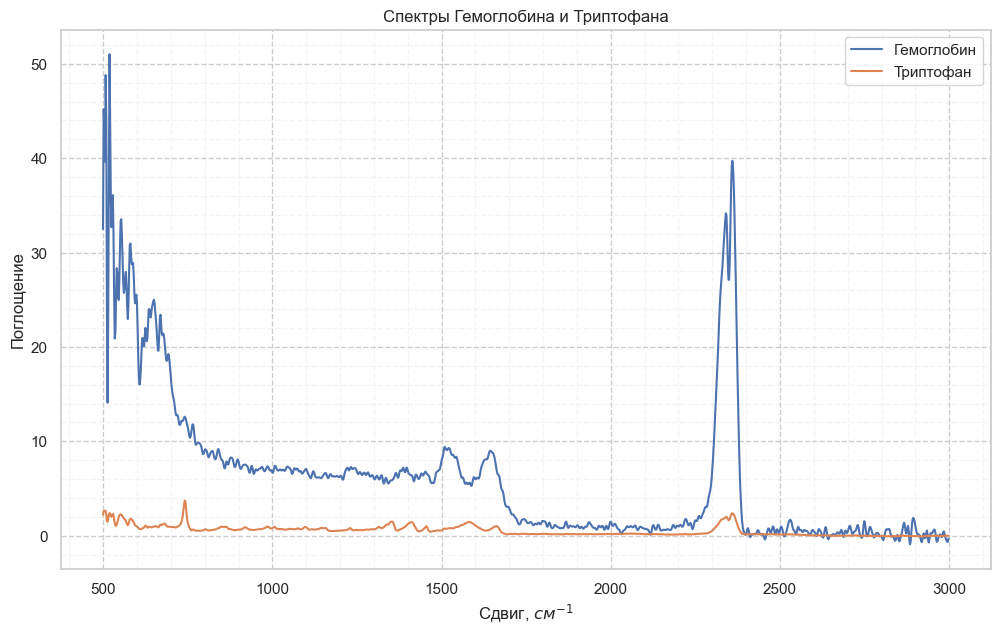
\includegraphics[width=0.7\linewidth]{Images/Гемоглобин и Триптофан.png}
    \caption{Спектры гемоглобины и триптофана}
    \label{гемоглобин и Триптофан}
\end{figure}

И последние спектры гемоглобина и триптофана (Рис. \ref{гемоглобин и Триптофан}).

В целом, два пика триптофана и у гемоглобина можно совместить. Таким образом, скорее всего в гемоглобине есть триптофан.

\textbf{Вторичная структура альбумина.}

Произведём анализ вторичной структуры альбумина по пику Амид I. Для этого построим график второй производной спектра в области Амид I и проведём анализ графика на пики. Далее была произведена коррекция базовой линии. Для определения соотношения составляющих вторичной структуры были посчитаны площади под графиком, которые почти соотносятся с данными из [2]. Результаты представлены на Рис. \ref{вторичная структура} и в Таблице \ref{tab:canonsummary}.

\begin{figure}[h!]
\centering
    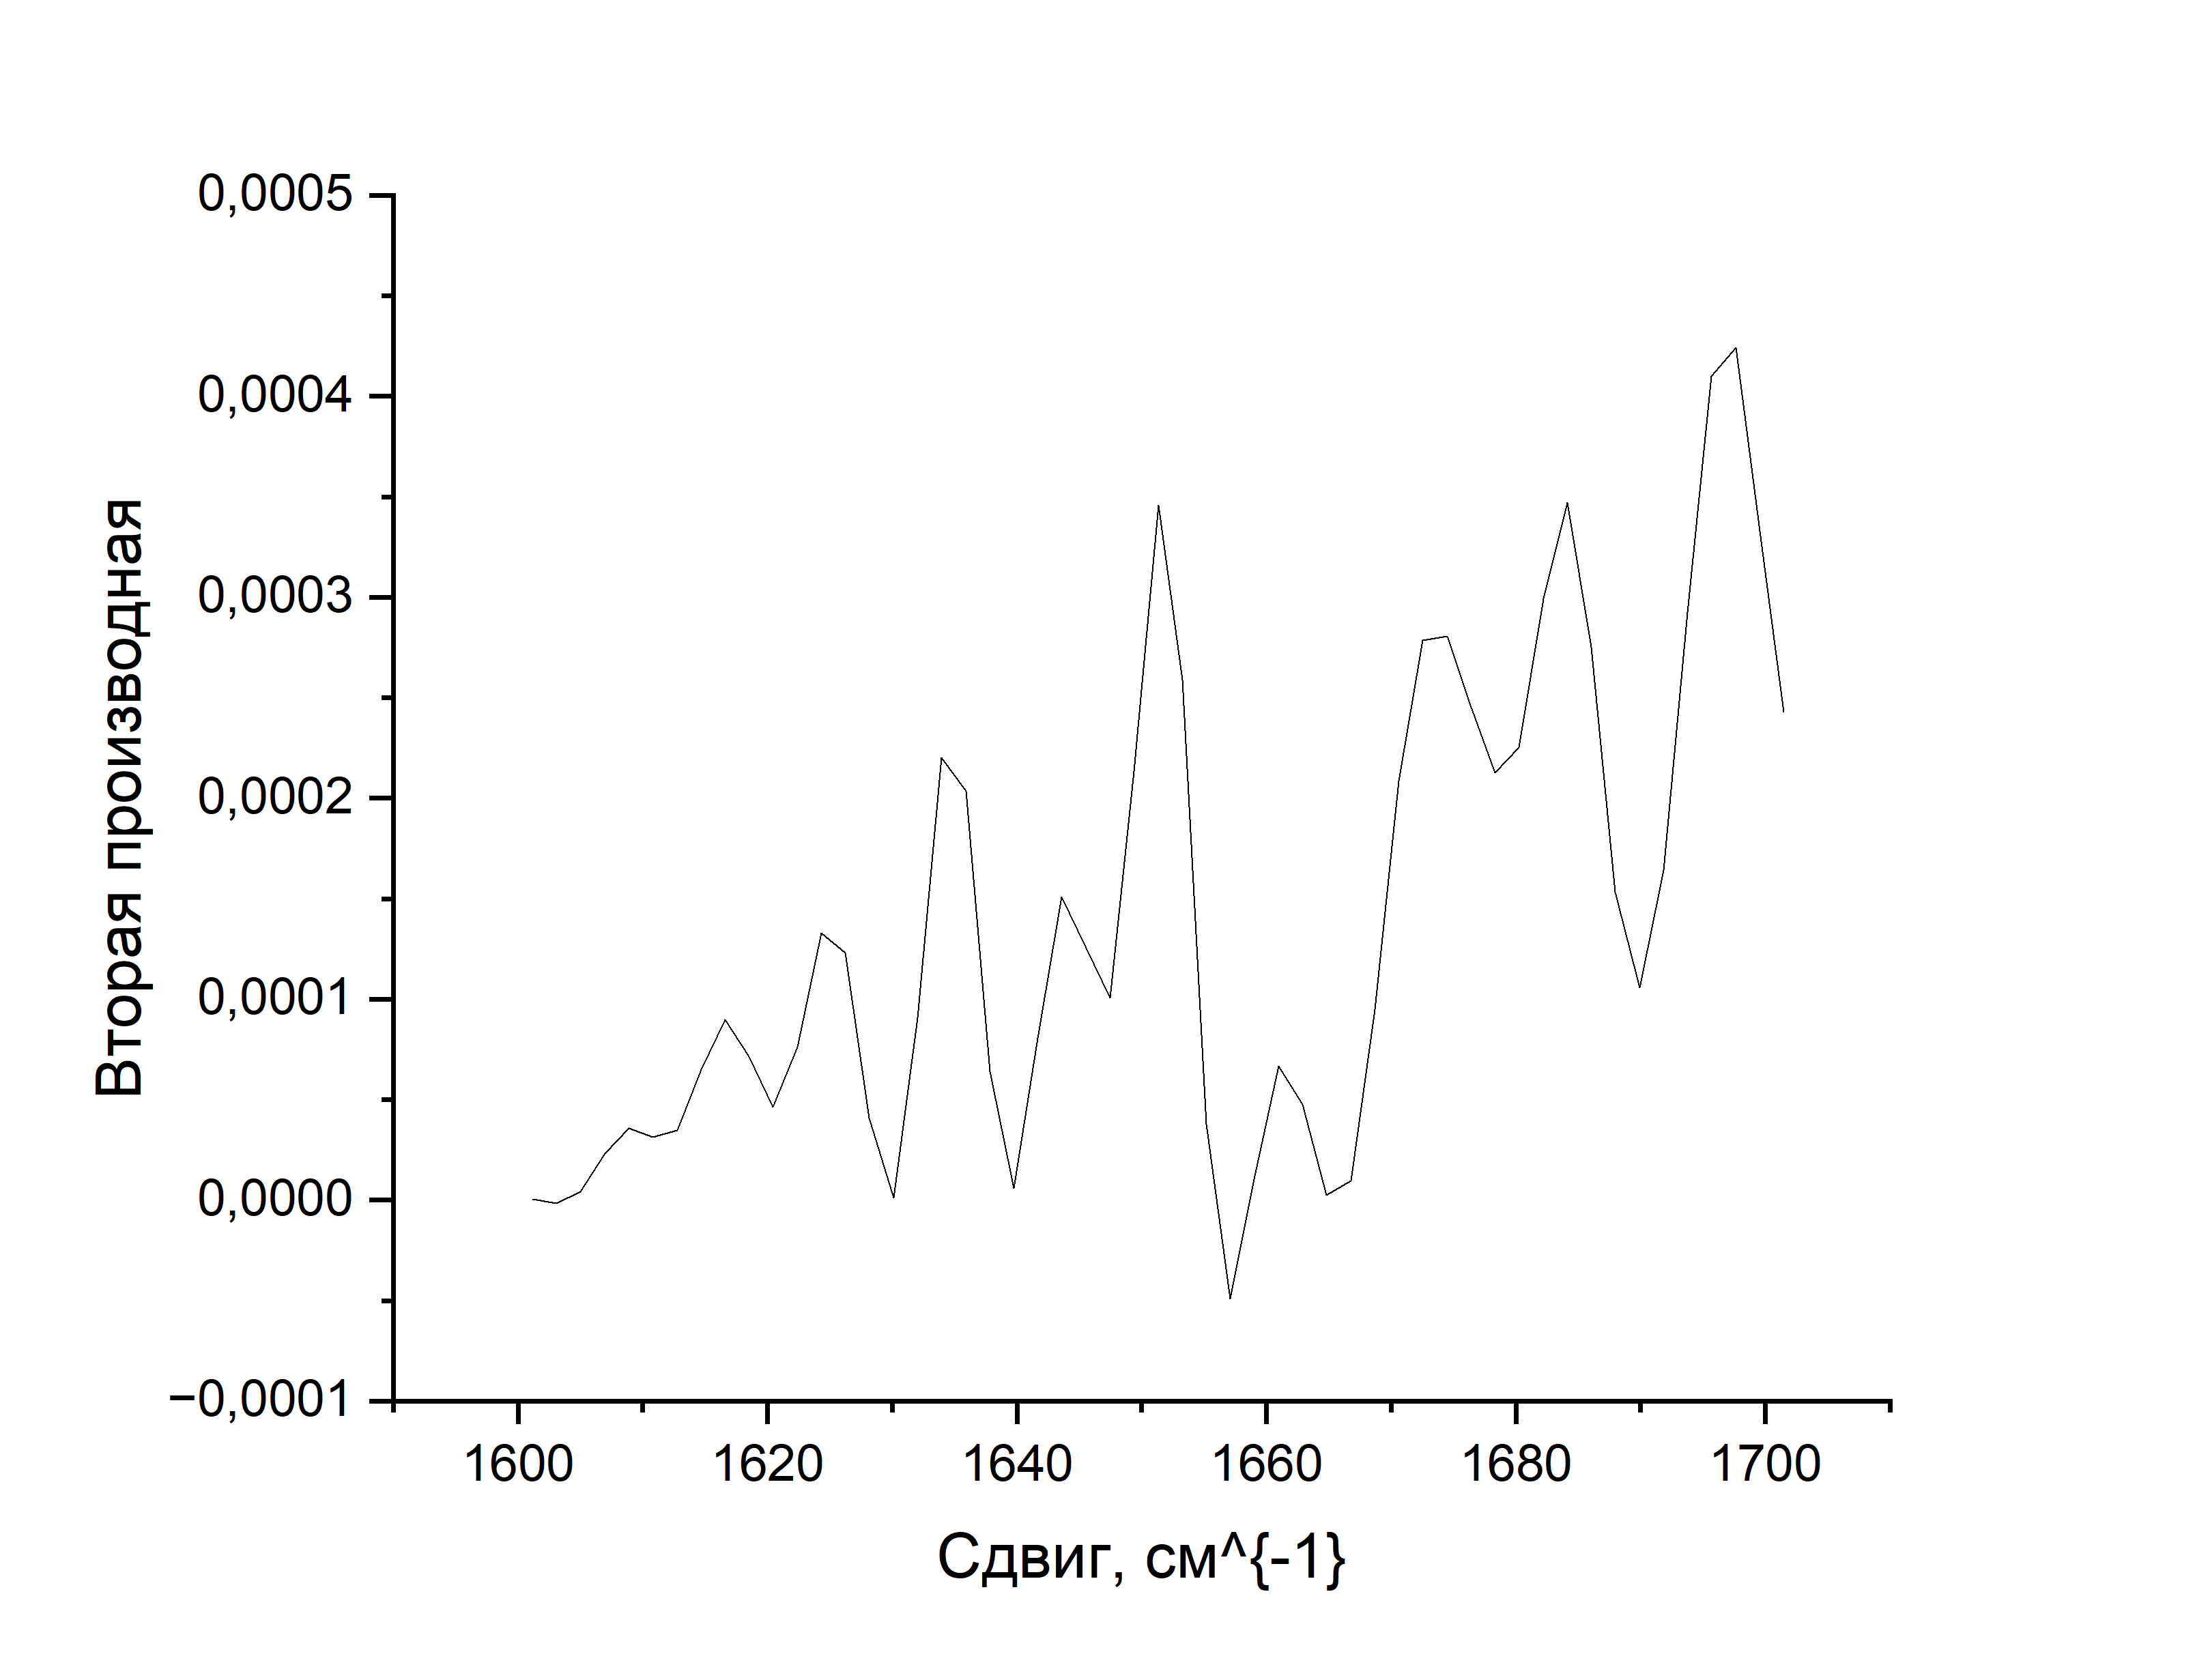
\includegraphics[width=0.7\linewidth]{Images/Вторичная структура БСА.png}
    \caption{Пики вторичной структурыс БСА}
    \label{вторичная структура}
\end{figure}

\begin{table}[h!]
\begin{center}
\caption{\label{tab:canonsummary} Процентное содержание структур в альбумине.}
\begin{tabular}{|c | c |} 
 \hline
 Структура & Площадь, \%   \\ [0.5ex] 
 \hline
 $\beta$ - поворот & 26,6  \\ 
 \hline
 $\beta$ - лист & 13,1  \\
 \hline
 $\alpha$ - спираль & 62,3   \\ [1ex] 
 \hline
\end{tabular}
\end{center}
\end{table}
\newpage
\subsection{Анализ спектра дерината}\;
\par Действующим веществом дерината является натрия дезоксирибонуклеат, также в состав входит вода и натрия хлорид. Удалось закристаллизовать двойную каплю дерината и снять спектр поглощения без плёнки. Сравним экспериментальный спектр (рис. \ref{деринат}) с эталонным (рис.\ref{эталон}).
\begin{figure}[h!] 
        \centering
        \minipage{0.5\textwidth}
        \centering
            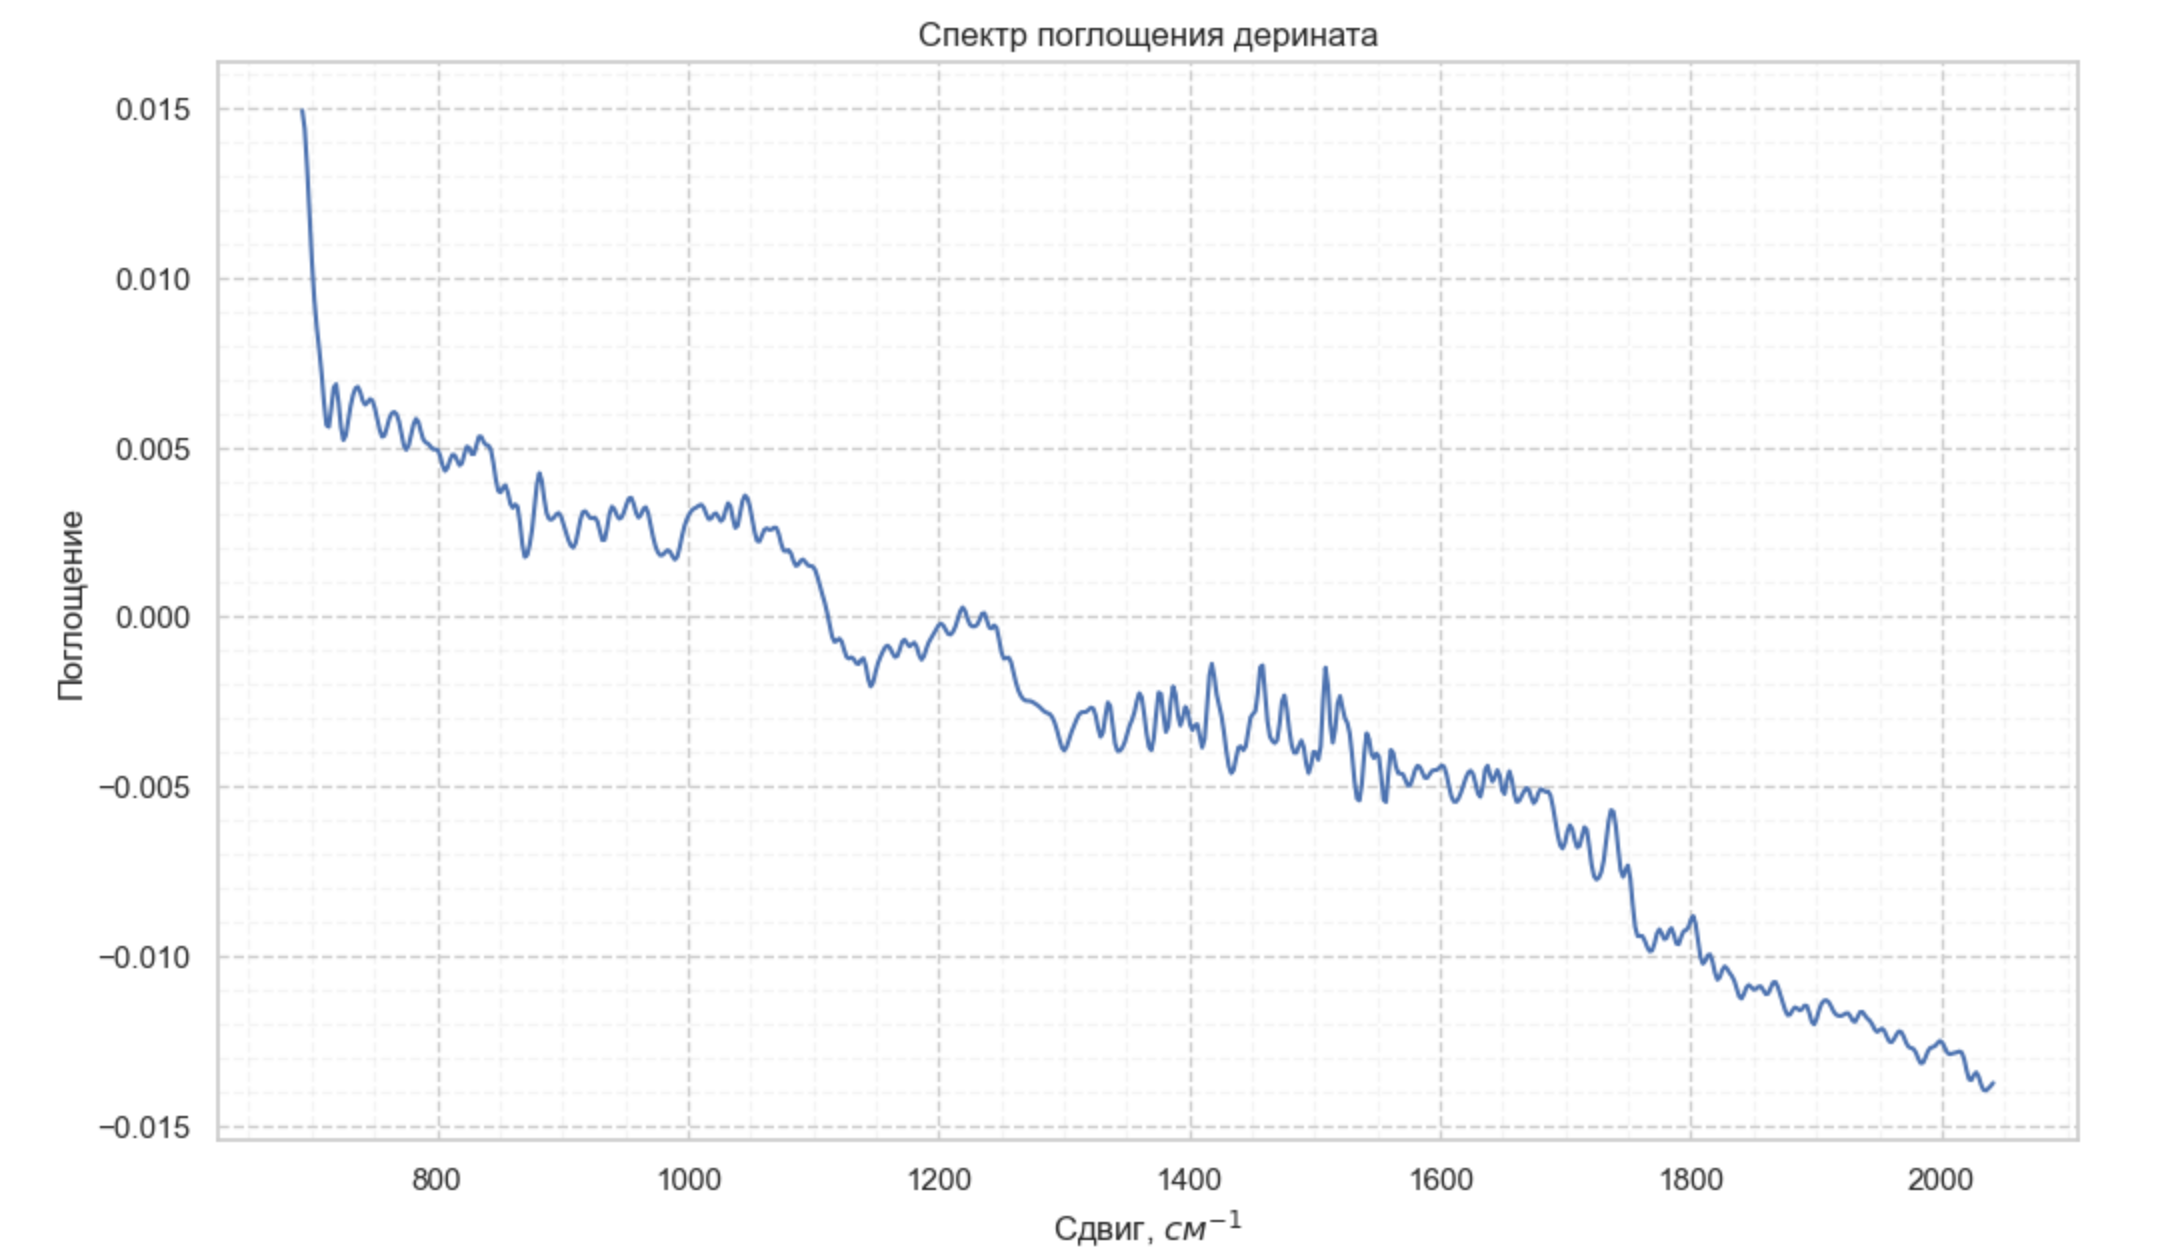
\includegraphics[width=0.9\linewidth]{Images/деринат.png}
                 \caption{Экспериментальный спектр поглощения дерината}
                 \label{деринат}
        \endminipage\hfill
        \minipage{0.5\textwidth}
        \centering
             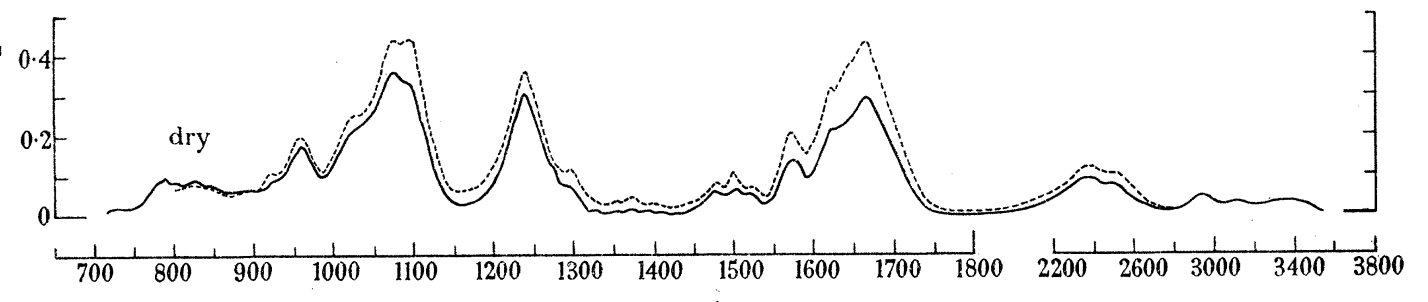
\includegraphics[width=0.9\linewidth]{Images/derinat.png}
                 \caption{Эталонный спектр поглощения дерината [3]}
                 \label{эталон}
        \endminipage
\end{figure}
\par Пики поглощения в эксперименте оказались не такими яркими, как для порошков. Однако пики в районе 1050 и 1250 $см^{-1}$ хорошо отличимы и совпадают с литературными данными на рис. \ref{эталон}. Пики в районе 1650 $см^{-1}$ различимы уже намного хуже.
\newpage
\subsection{Спектр поглощения паров соляной кислоты}\;
\par Для регистрации спектра паров соляной кислоты (рис. \ref{HCl}) приставка в установке была заменена на штатив с разогретой трубкой, заполненной газообразным HCl. 
\begin{figure}[h!]
\centering
    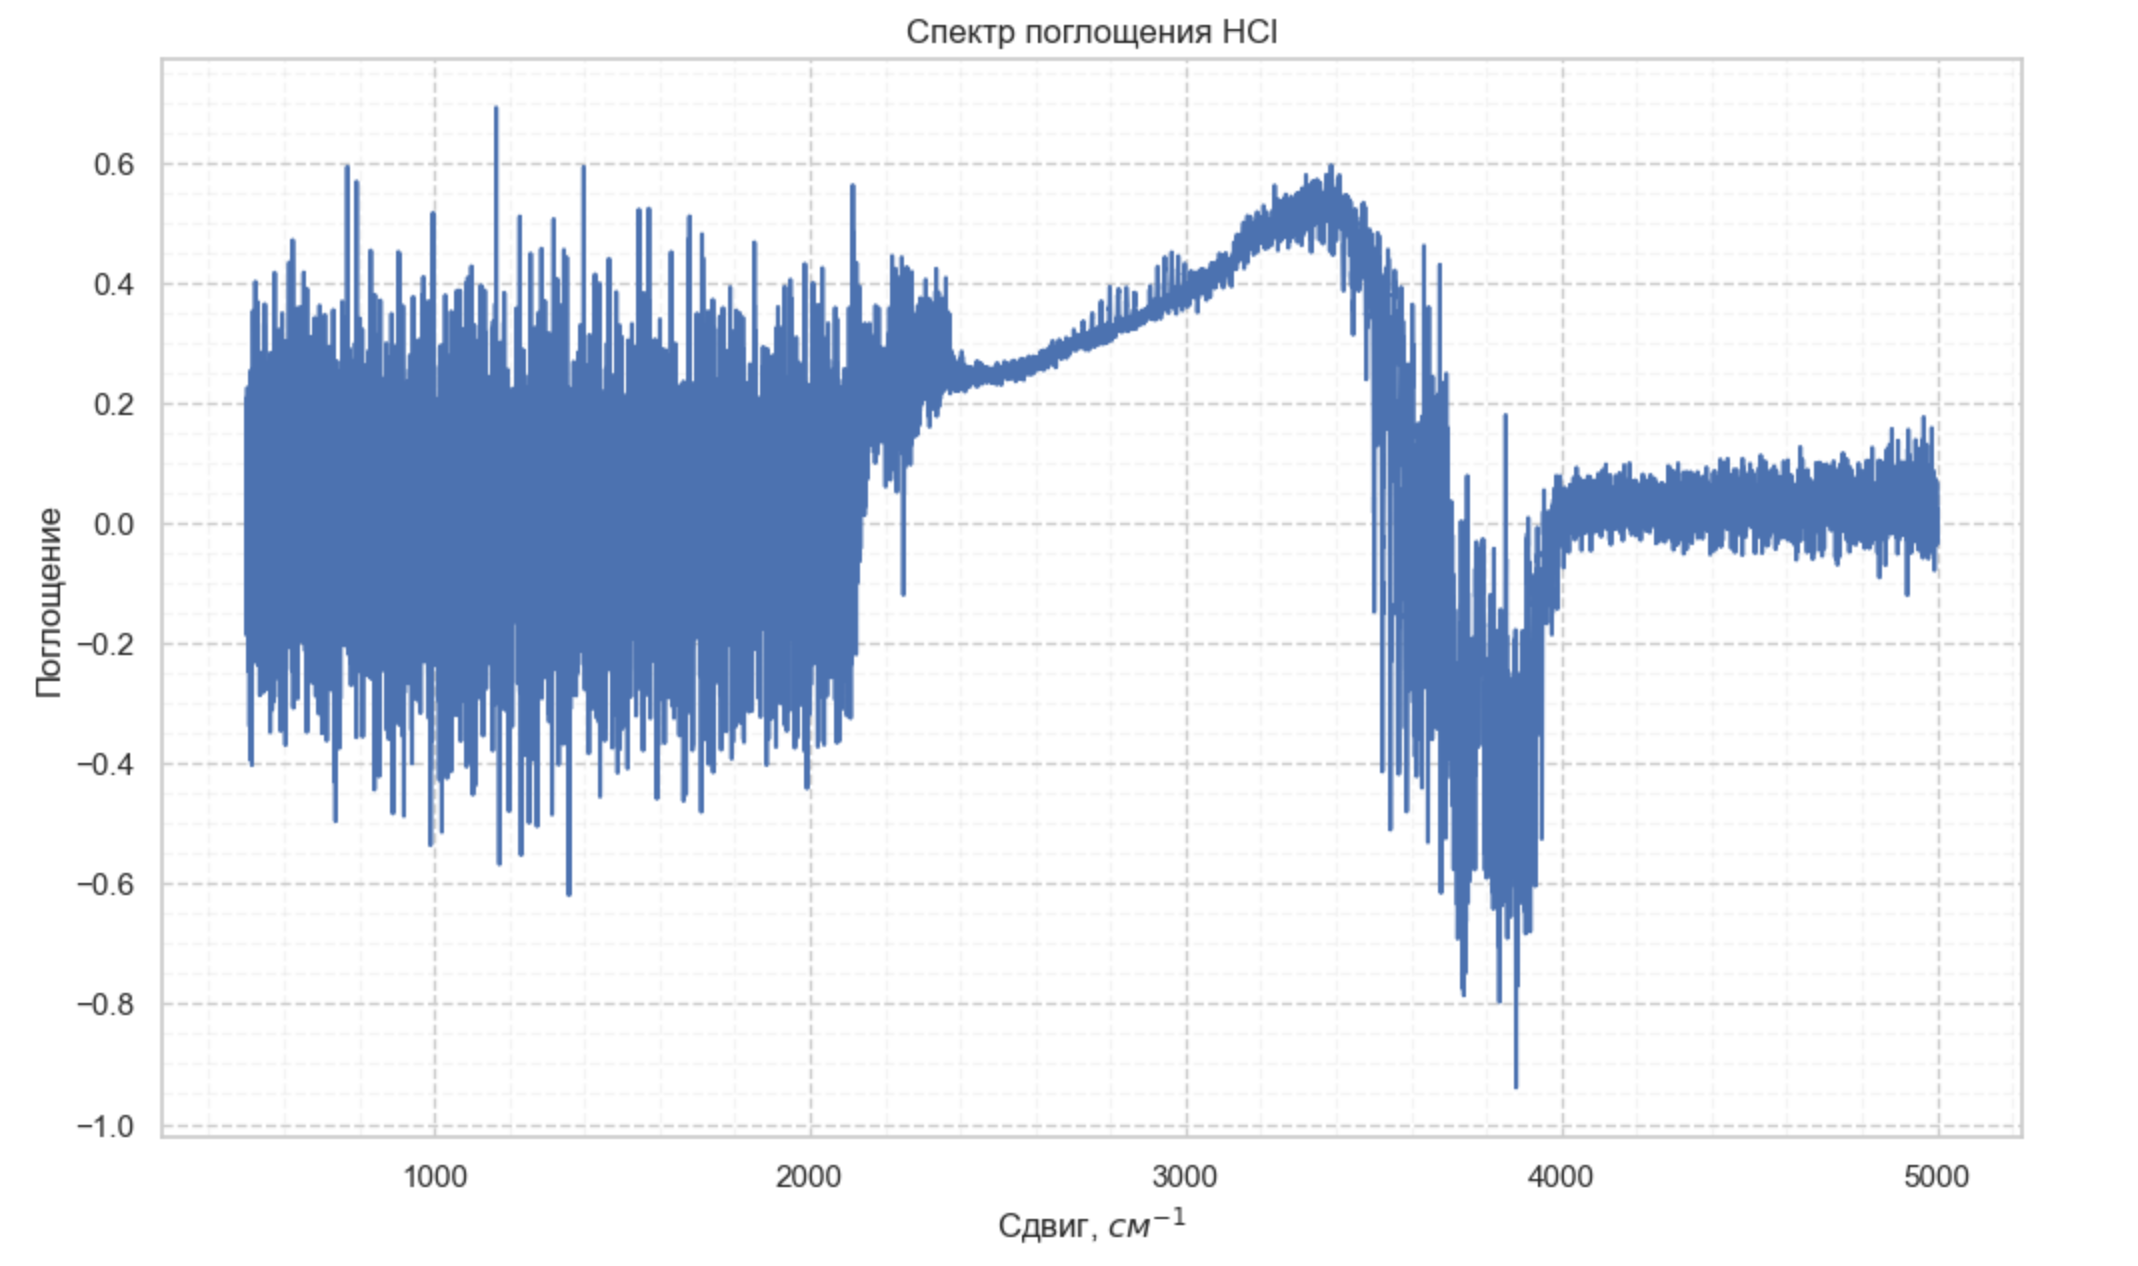
\includegraphics[width=0.8\linewidth]{Images/HCl.png}
    \caption{Спектр поглощения паров соляной кислоты}
    \label{HCl}
\end{figure}
\begin{figure}[h!]
\centering
    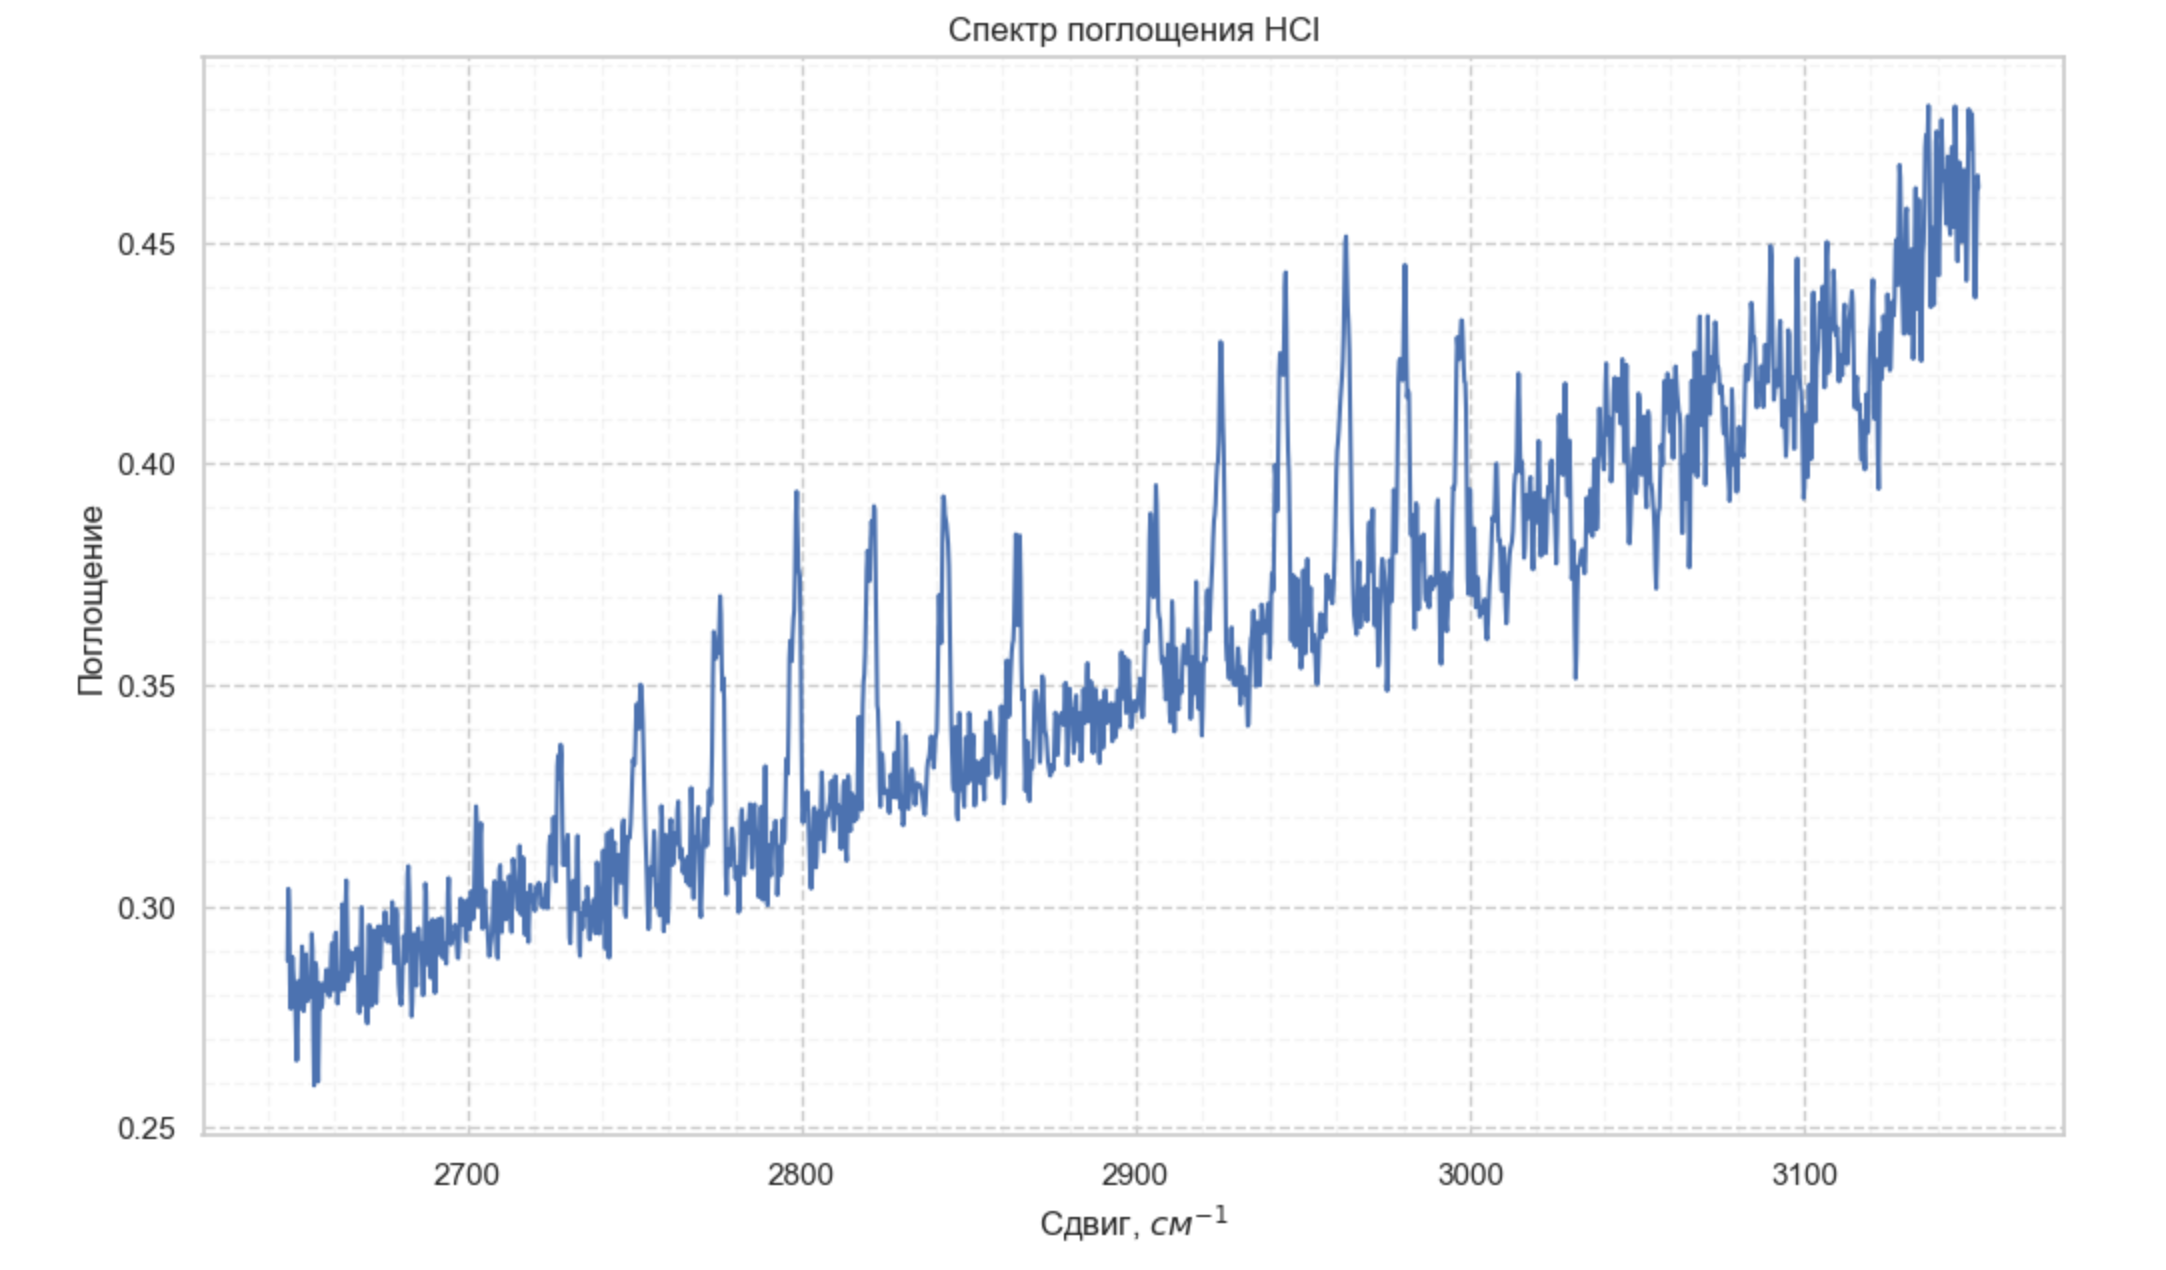
\includegraphics[width=0.8\linewidth]{Images/ветви.png}
    \caption{P-ветви (слева) и R-ветви (справа) на спектре поглощения HCl}
    \label{ветви}
\end{figure}
\par На спектре хлороводорода в диапазоне 2700-3000 $см^{-1}$ заметны P и R-ветви, причём с увеличением квантового числа интенсивность вращательных линий сначала возрастает (из-за
линейного роста степени вырождения вращательных уровней), а потом постепенно падает (из-за низкой заселённости высоких энергетических уровней).
\newpage
\section{Выводы}
\begin{itemize}
    \item В ходе выполнения работы столкнулись с особенностями работы установки, в результате чего модифицировали методику регистрации пиков на спектре поглощения. Пики, соответсвующие поглощению клейкой основы зарегистрированы не были, поэтому при обработке нормировка не использовалась.
    \item В ходе работы был проведён анализ спектров белков (БСА и гемоглобина), также сравнительный анализ спектров белков и триптофан. Полученные значения частот попадают в теоретические диапазоны из приведённых источников.
    \item Дополнительно, был изучен спектр альбумина для определения его вторичной структуры с помощью второй производной. Приведённые соотношения вполне соответствуют литературным данным.
    \item Был получен спектр поглощения дерината (натрия дезоксирибонуклеата) - основные пики поглощения совпали с литературными данными.
    \item На спектре поглощения паров соляной кислоты были зарегистрированы P- и R-ветви колебательно-вращательных полос, причём с увеличением квантового числа интенсивность вращательных линий сначала возрастает, а потом постепенно падает.
\end{itemize}

\section{Список литературы.}
\begin{enumerate}
    \item Kong J, Yu S. Fourier transform infrared spectroscopic analysis of protein secondary structures. Acta Biochim Biophys Sin (Shanghai). 2007 Aug;39(8):549-59. doi: 10.1111/j.1745-7270.2007.00320.x. PMID: 17687489.   
    \item Усольцев Д. А., Ситникова В. Е., Носенко Т. Н., Олехнович Р. О., Успенская М. В. Сравнение методик расчета вторичной структуры белков на основе деконволюции инфракрасных спектров // Научно-технический вестник информационных технологий, механики и оптики. 2019. №4. 
    \item Gordon Brims Black Mcivor Sutherland and M. Tsuboi. The infra-red spectrum and molecular configuration of sodium deoxyribonucleate, 451 (1957).
\end{enumerate}
\end{document}
